\section{Modelagem Empírica}
\label{sec:modemp}

\subsection{Dados}

A principal fonte de dados públicos sobre sinistros de trânsito em São Paulo é o Infosiga (Sistema de Informações Gerenciais de Acidentes de Trânsito do Estado de São Paulo), um sistema criado em 2016 e gerenciado pelo Detran-SP. A proposta, quando foi criado, era de apresentar dados de óbitos e acidentes com vítimas, atualizados mensalmente \cite{Res_SG-6_de_23-2-2016}, mas o levantamento de sinistros sem vítimas fatais passou a ser realizado apenas a partir de 2019. Os dados do Infosiga são coletados a partir da base de dados do RDO (Registro de Ocorrências), sistema usado pela polícia para registrar os Boletins de Ocorrência (BOs) em escala estadual \cite{plano_segviar}. A partir da análise desses BOs, os dados são tabulados e registrados, dessa forma, caso não haja um BO sobre o acidente, ele não constará na base de dados. 

É importante ressaltar que quando há vítimas envolvidas no sinistro, independentemente da natureza da lesão, registrar o BO é uma norma, cujo descumprimento leva à uma multa gravíssima, de acordo com o Art. 176 do Código de Trânsito Brasileiro (CTB). Ademais, mesmo quando não obrigatório -- em cenários de sinistros sem vítimas --, o BO pode ser requerido em diversas situações, como pela seguradora, caso seu serviço seja necessário. Quando o sinistro resulta em óbito, é necessário que se faça um BO para enterrar a vítima. Dessa forma, é de se esperar que, para sinistros graves ou que envolvam óbitos, não haja subnotificações. Ao passo que a gravidade diminui, há menores chances de que seja feito o BO e que o evento conste na base de dados. A figura \ref{fig:fluxograma} ajuda a compreender os cenários em que os dados estão mais completos.

\begin{figure}[h]
    \centering
    \caption{Fluxograma de notificação de um sinistro}
    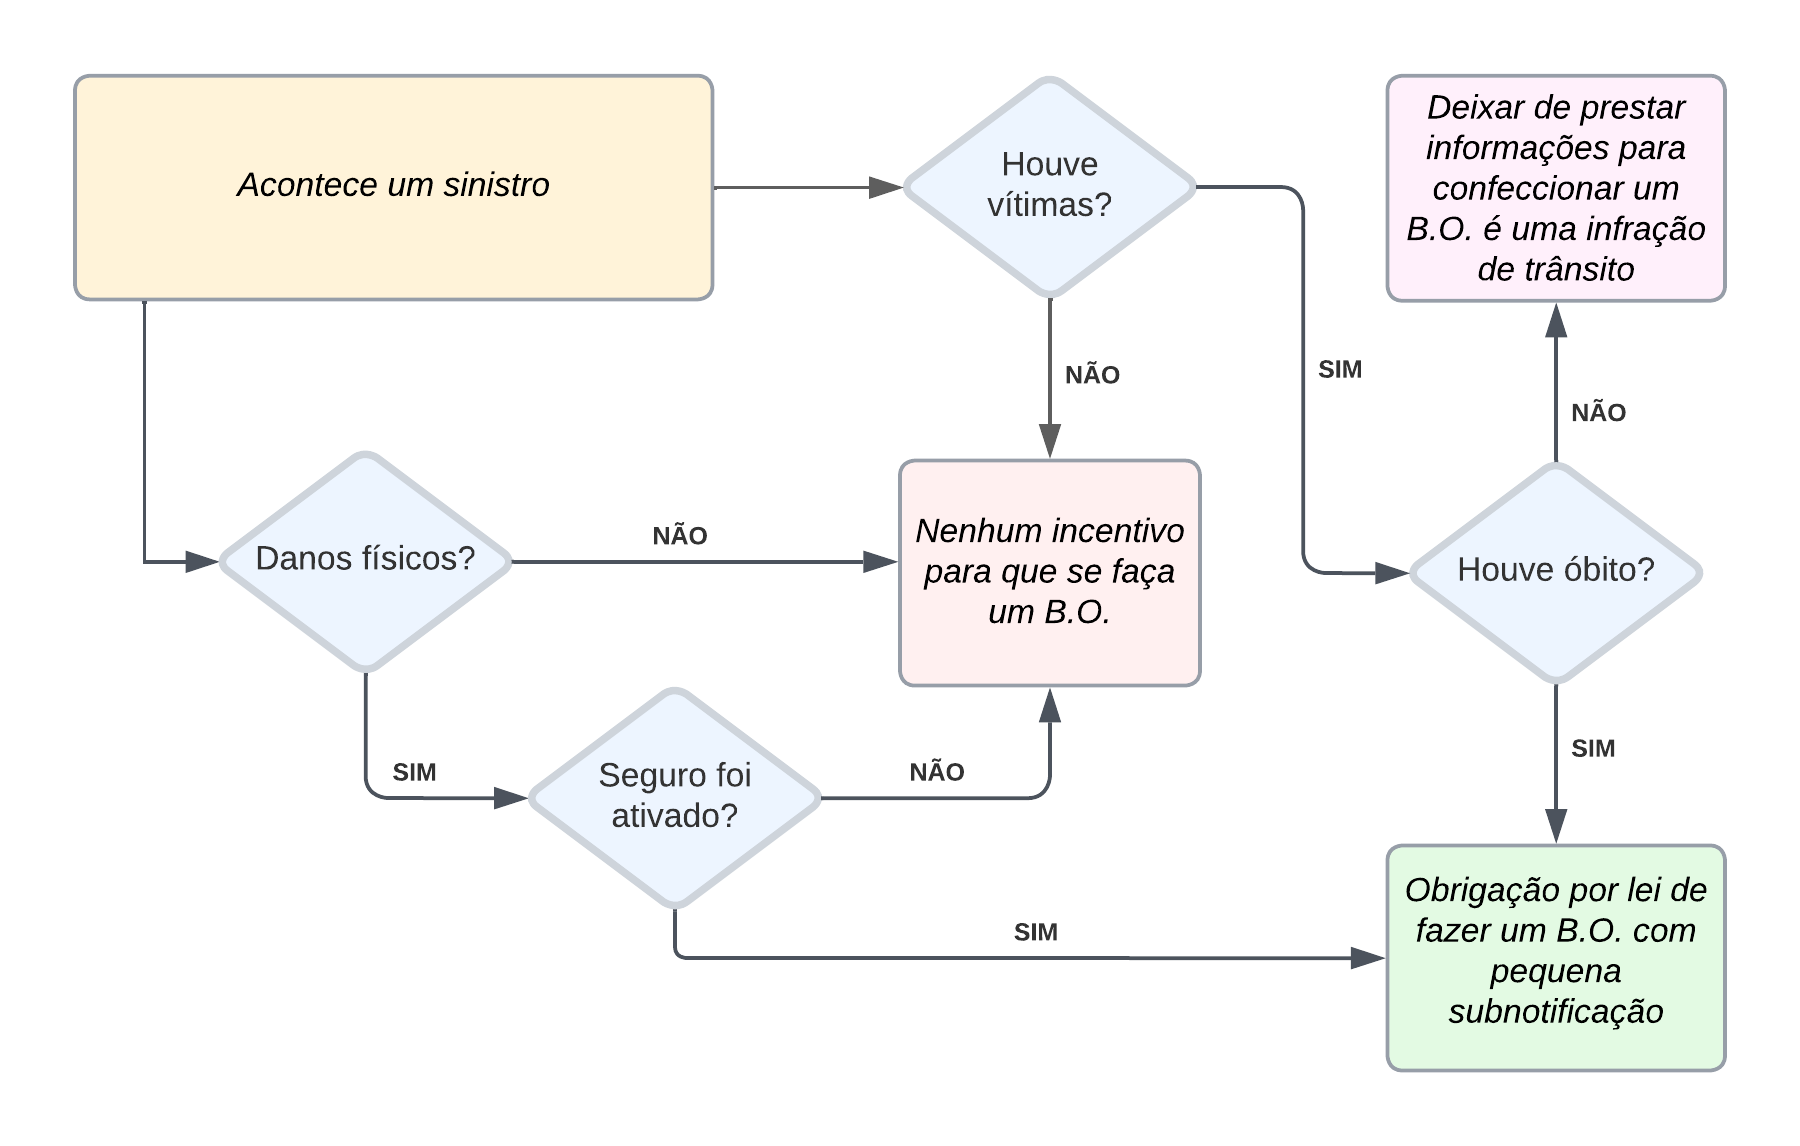
\includegraphics[width = 0.85\linewidth]{relatorios/faixa-azul/figuras/fluxograma.png}
    \label{fig:fluxograma}
\end{figure}

Há outras fontes de dados que devem também ser mencionadas, sendo que em escala federal há apenas três \cite{magaly2011}. O Sistema de Informação sobre Mortalidade (SIM), criado pelo DATASUS, do Ministério da Saúde, divulga informações sobre vítimas de sinistros de trânsito que passaram pelo SUS. O Registro Nacional de Acidentes e Estatísticas de Trânsito (Renaest), sob a coordenação do Departamento Nacional de Trânsito (Denatran) organiza e junta os dados dos Detrans de cada unidade federativa \cite{nogueira2016morte}. Por fim o DPVAT é um seguro obrigatório que existe desde 1974 para a cobertura de danos pessoais causados por sinistros de trânsito, cujos dados são divulgados trimestralmente através de relatórios. O comparativo entre as bases se encontra no Anexo \ref{anx:comparativo}, mas em suma, os dados do Infosiga são mais completos e são a escolha para este estudo.

Na seção do anexo \ref{anx:infosiga} foi feita uma análise mais aprofundada da base dados, que apresenta algumas limitações dos dados, bem como sugestões de melhor organização dessa base. Em seguida se encontra a descrição apenas das variáveis utilizadas na pesquisa:

\begin{itemize}
    \item Data do Sinistro: Inclui ano, mês, dia e horário do sinistro.
    \item Logradouro e número: Endereço e número do local em que o sinistro ocorreu, da forma como foi registrada no BO.
    \item Veículos Envolvidos: Existe uma coluna para cada tipo de veículo, em que os valores são binários (o veículo estava presente no sinistro ou não). As possibilidades são automóvel, motocicleta, pedestre, bicicleta, caminhão, ônibus e outros.    
    \item Pessoas Envolvidas: Existem 3 colunas desse tipo, relacionadas a gravidade do quadro clínico, podendo ser ileso, leve ou grave. Em cada coluna é apresentada a quantidade de pessoas que apresentavam a gravidade em questão no sinistro.     
\end{itemize}

Os dados então foram filtrados, agregados e organizados e receberam ajustes pontuais\footnote{Como é possível observar na Figura \ref{fig:sinistros}, o mês de março de 2023 apresenta zero sinistros de carros e caminhões no município de São Paulo, o que é impossível. Nesse sentido, considerando que isso é um erro na base de dados, os dados desse mês foram interpolados utilizando a média dos três meses anteriores.}. Foram considerados apenas os sinistros no município de São Paulo, que envolveram ao menos um motociclistas e que deixaram ao menos um ferido (grave ou leve), de forma a minimizar o viés de sub-notificação, como demonstrado na Figura \ref{fig:fluxograma}. Depois, os dados foram agregados por avenida e mês, resultando em um número de sinistros para esse par de chaves únicas. Entretanto, como comentado na Seção \ref{sec:modteor}, o comportamento no trânsito é muito caótico, levando a série a apresentar muito ruído -- que prejudica a análise. Para lidar com isso, aplicou-se a raiz quadrada e o filtro Hodrick-Prescott (HP) com o objetivo de isolar as tendências de longo prazo dos componentes cíclicos de curto prazo nos dados de sinistros, além de estabilizar a variância e diminuir o efeito de \textit{outliers}. O resultado desse procedimento para a Avenida Bandeirantes pode ser observado na Figura \ref{fig:bandeirantes}.

\begin{figure}[h]
    \centering
    \caption{Sinistros na Avenida dos Bandeirantes}
    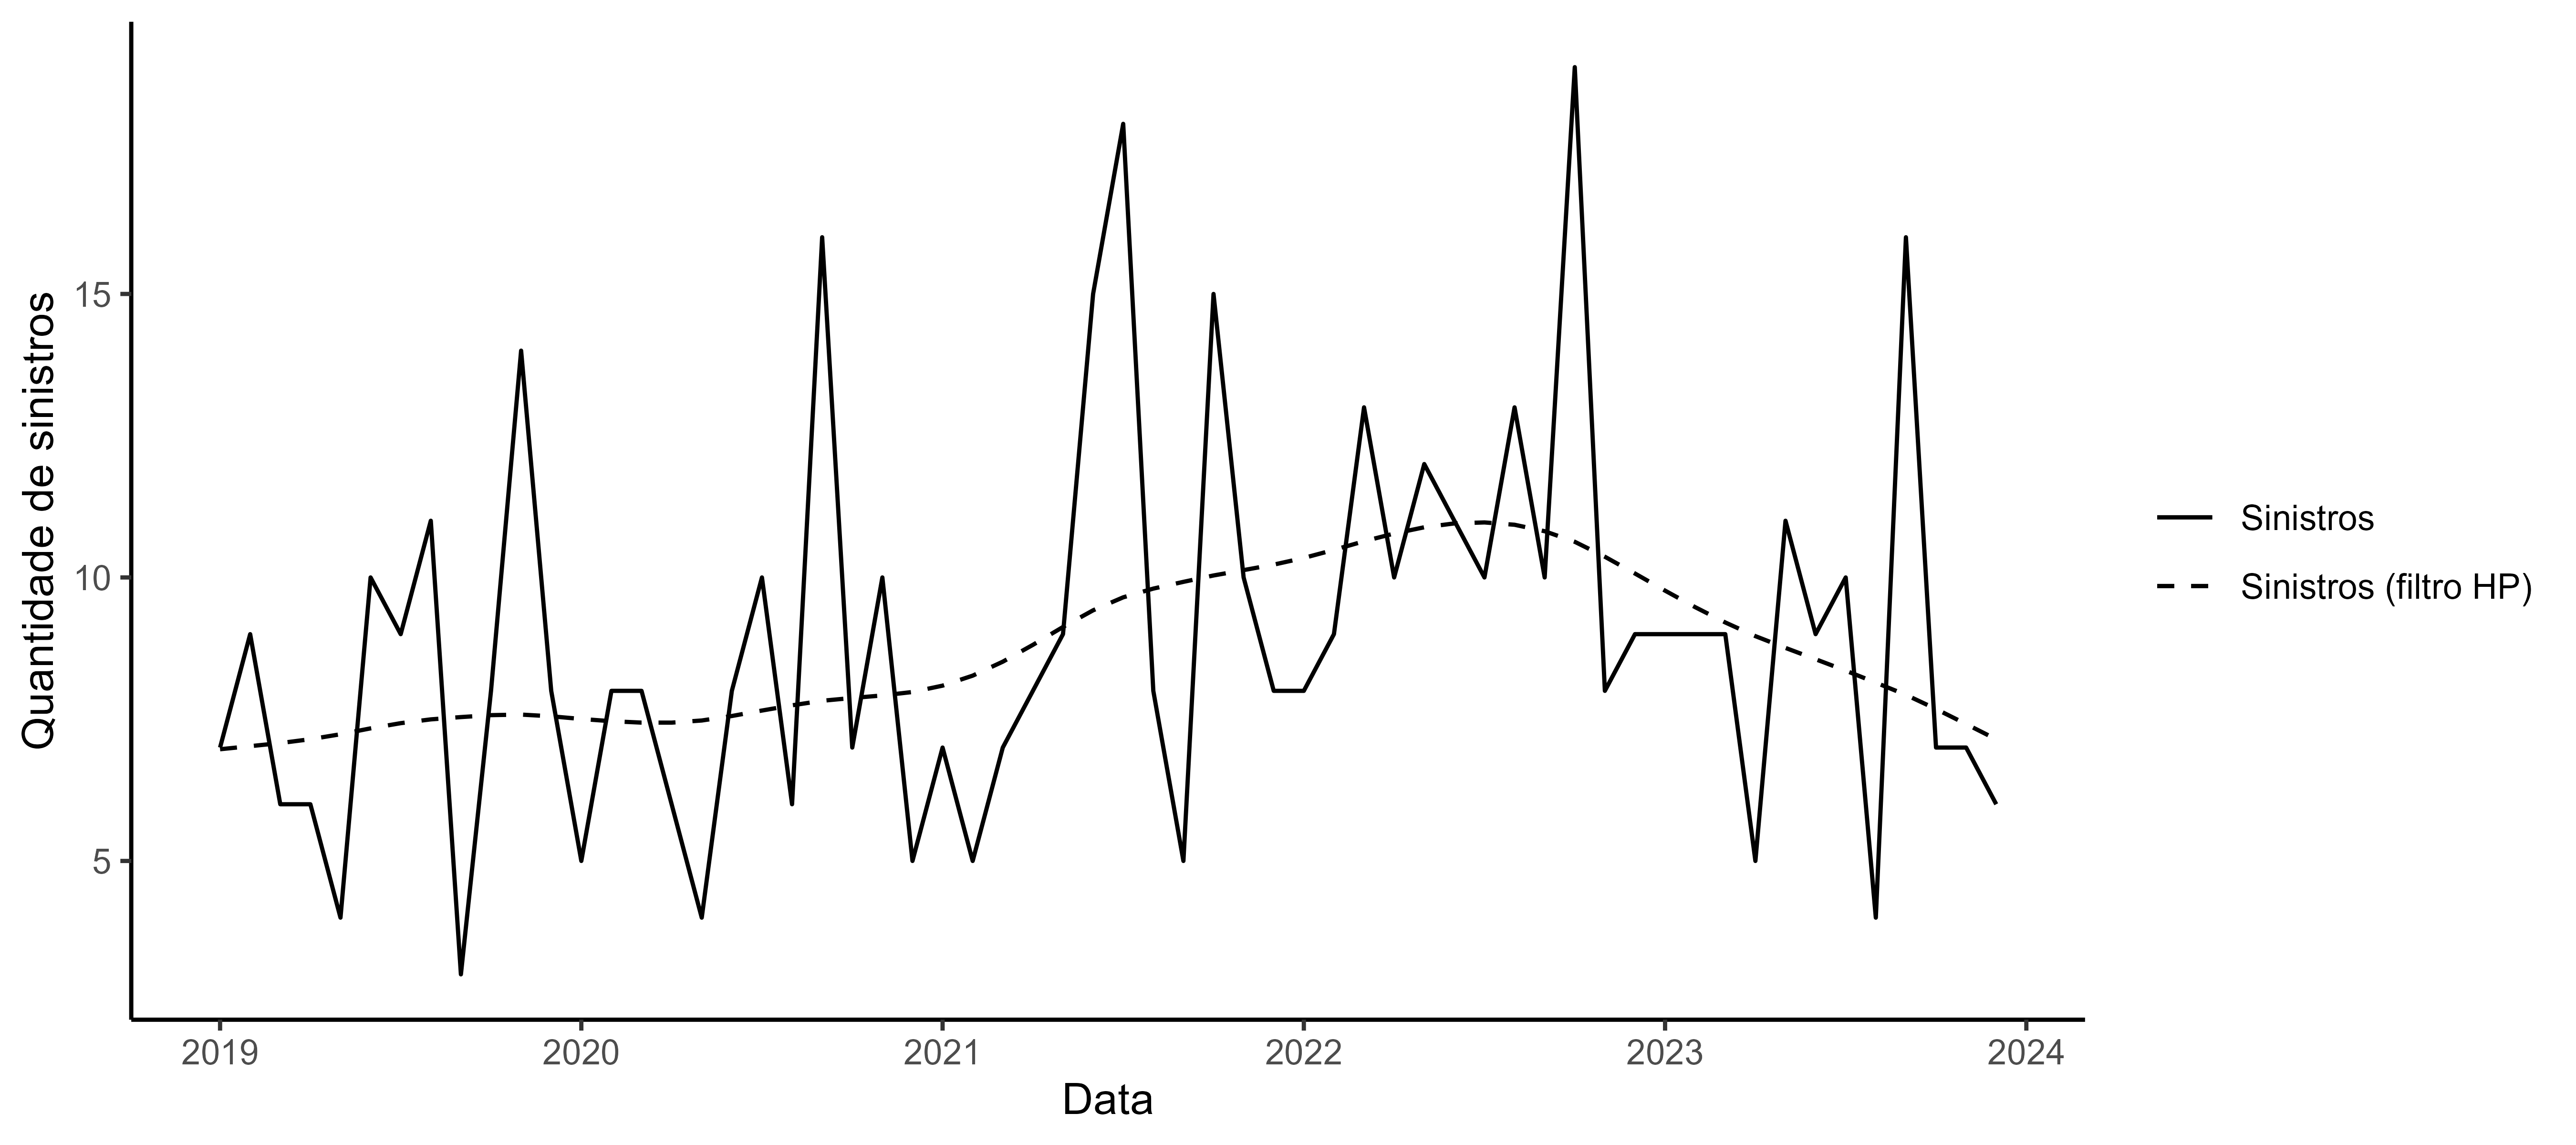
\includegraphics[width = 0.8\linewidth]{relatorios/faixa-azul/figuras/FiltroHP.png}
    \label{fig:bandeirantes}
\end{figure}

A Avenida 23 de Maio, apesar de ser a primeira a receber o tratamento, apresentou faixa azul apenas em um sentido, mas na base de dados do Infosiga não é discriminado em qual sentido da via ocorreu o sinistro, impossibilitando que a análise seja feita sobre ela. A Avenida dos Bandeirantes foi implementada poucos meses depois, em sua completude, sendo o caso perfeito para este estudo. Em 2023 outras faixas azuis começaram a surgir, mas dado que foram implementadas apenas recentemente, não há meses suficientes para que seja feita uma análise robusta. Dessa forma, a única unidade tratada na análise é a Av. dos Bandeirantes.

Em relação aos dados de fluxo de veículos, a CET-SP divulga anualmente um relatório contendo a lentidão de trechos de vias de grande circulação em São Paulo. Esses dados são coletados a partir dos radares espalhados pelas vias e a Avenida 23 de Maio, por exemplo, está categorizada junto com a Avenida Rubem Berta e Avenida Moreira Guimarães, apresenta diferentes trechos: da rua Aratâs até o Viaduto João João Julião da Costa Águiar, do Viaduto da Rua Pedroso até o Terminal Bandeira, do Viaduto General Euclides de Figueiredo até a Avenida Indianópolis, entre outros. Ademais, a lentidão dos trechos está separada para o sentido da via, e, no caso da Av. 23 de Maio, é separado por Santana ao Aeroporto ou o contrário. 

Todavia, a base de dados apresenta uma série de problemas que impossibilitam sua utilização. Primeiramente, as ruas não apresentam um código identificador que possa ser cruzado com outra base e os nomes estão escritos de maneira inconsistente e que pode variar de ano para ano. A medida apresentada de ``lentidão'' não tem seu significado apresentado nem uma metodologia de como é calculada, tornando-a uma variável sem muito valor. Ademais, os valores estão incompletos, apresentando grandes períodos em que não há dados. Por fim, a separação de trechos é feita de tal forma que uma única avenida pode apresentar dezenas ou centenas de trechos, impossibilitando que se identifique um trecho que represente a avenida como um todo, dado que é necessário fazer esse processo para um grande contingente de avenidas.


\subsection{Identificação}

Para fazer a identificação causal do efeito da faixa azul, o método escolhido neste estudo foi o de controle sintético, apresentando como principal referência as contribuições de \textcite{abadie2010synthetic}. A escolha por esse método se encontra no fato de haver apenas uma unidade amostral tratada. Essa abordagem envolveu a criação de uma versão sintética da Avenida Bandeirantes, uma das principais vias de São Paulo. A Avenida Bandeirantes sintética foi modelada a partir de uma combinação linear de dezenas de outras grandes vias urbanas que não receberam a implementação da faixa azul, mas que possuem características semelhantes em termos de tráfego, estrutura urbana, e outros fatores relevantes. 

\begin{figure}[h]
    \caption{Construção do controle sintético}
    \begin{subfigure}[t]{0.45\linewidth}
        \centering
        \caption{Componentes da Bandeirantes sintética}
        \begin{adjustbox}{width = \linewidth}
            \begin{tiny}
    \centering
\begin{tabular}{p{0.45\textwidth}p{0.15\textwidth}}
\hline
Nome da Via & Peso \\ 
  \hline
Av. Mutinga & 30.26\% \\ 
Sp 015 & 20.23\% \\ 
Ace. Estr. do M'Boi Mirim & 05.59\% \\ 
Sp 270 & 01.74\% \\ 
Av. Sen. Teotônio Vilela & 01.41\% \\
Estr. De Itapecerica & 01.14\% \\
Av. Sapopemba & 01.26\% \\ 
Av. Aricanduva & 01.17\% \\ 
Av. Atlântica & 01.06\% \\
Av. Washington Luis & 01.01\% \\
Av. Interlagos & 00.96\% \\ 
Estr. Do Campo Limpo & 00.82\% \\ 
Outras avenidas & 33.70\%
 
\end{tabular}
\end{tiny}
        \end{adjustbox}
        \label{fig:bandeirantes_sintetica}
    \end{subfigure}
    \hfill
    \begin{subfigure}[t]{0.45\linewidth}
        \centering
        \caption{Av. Bandeirantes (laranja) e SP015 (vermelha)}
        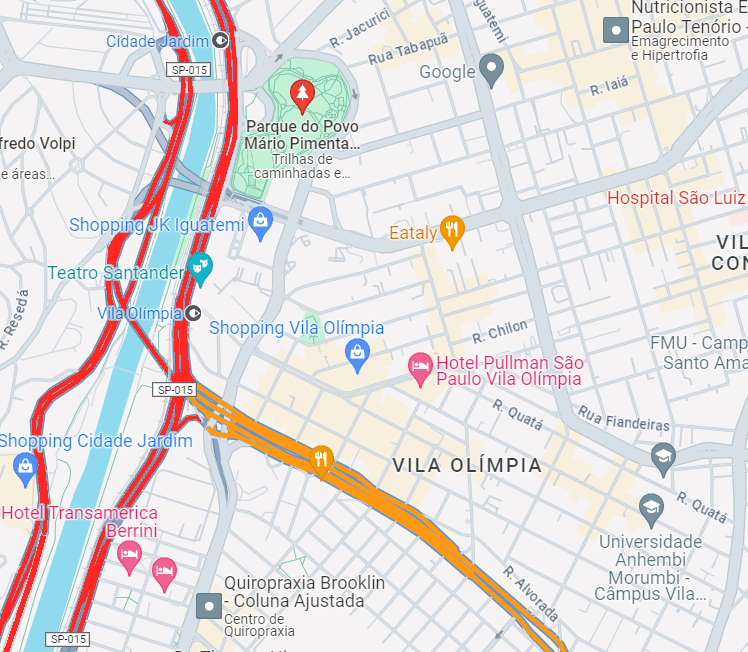
\includegraphics[width=.8\linewidth]{relatorios/faixa-azul/figuras/band.png}
        \label{fig:sp015}
    \end{subfigure}
\end{figure}

A escolha de quais avenidas e qual peso cada uma delas apresenta no controle sintético é calculado automaticamente pelo método, de forma a minimizar a diferença entre a Bandeirantes observada (real) e a sintética antes do período de tratamento. Os principais componentes da Bandeirantes sintética podem ser visualizadas na Figura \ref{fig:bandeirantes_sintetica}. Vale salientar que a SP 015, segundo componente mais relevante, é uma continuação física da Av. dos Bandeirantes (Figura \ref{fig:sp015}), que troca de nome depois de um viaduto. Isso é uma evidência qualitativa de que o método acabou por escolher uma avenida que compartilha de muitas características com a Av. dos Bandeirantes, a não ser o fato de receber o tratamento. Evidências quantitativas serão discutidas adiante.

\begin{figure}[h]
    \centering
    \caption{Bandeirantes observada e sintética}
    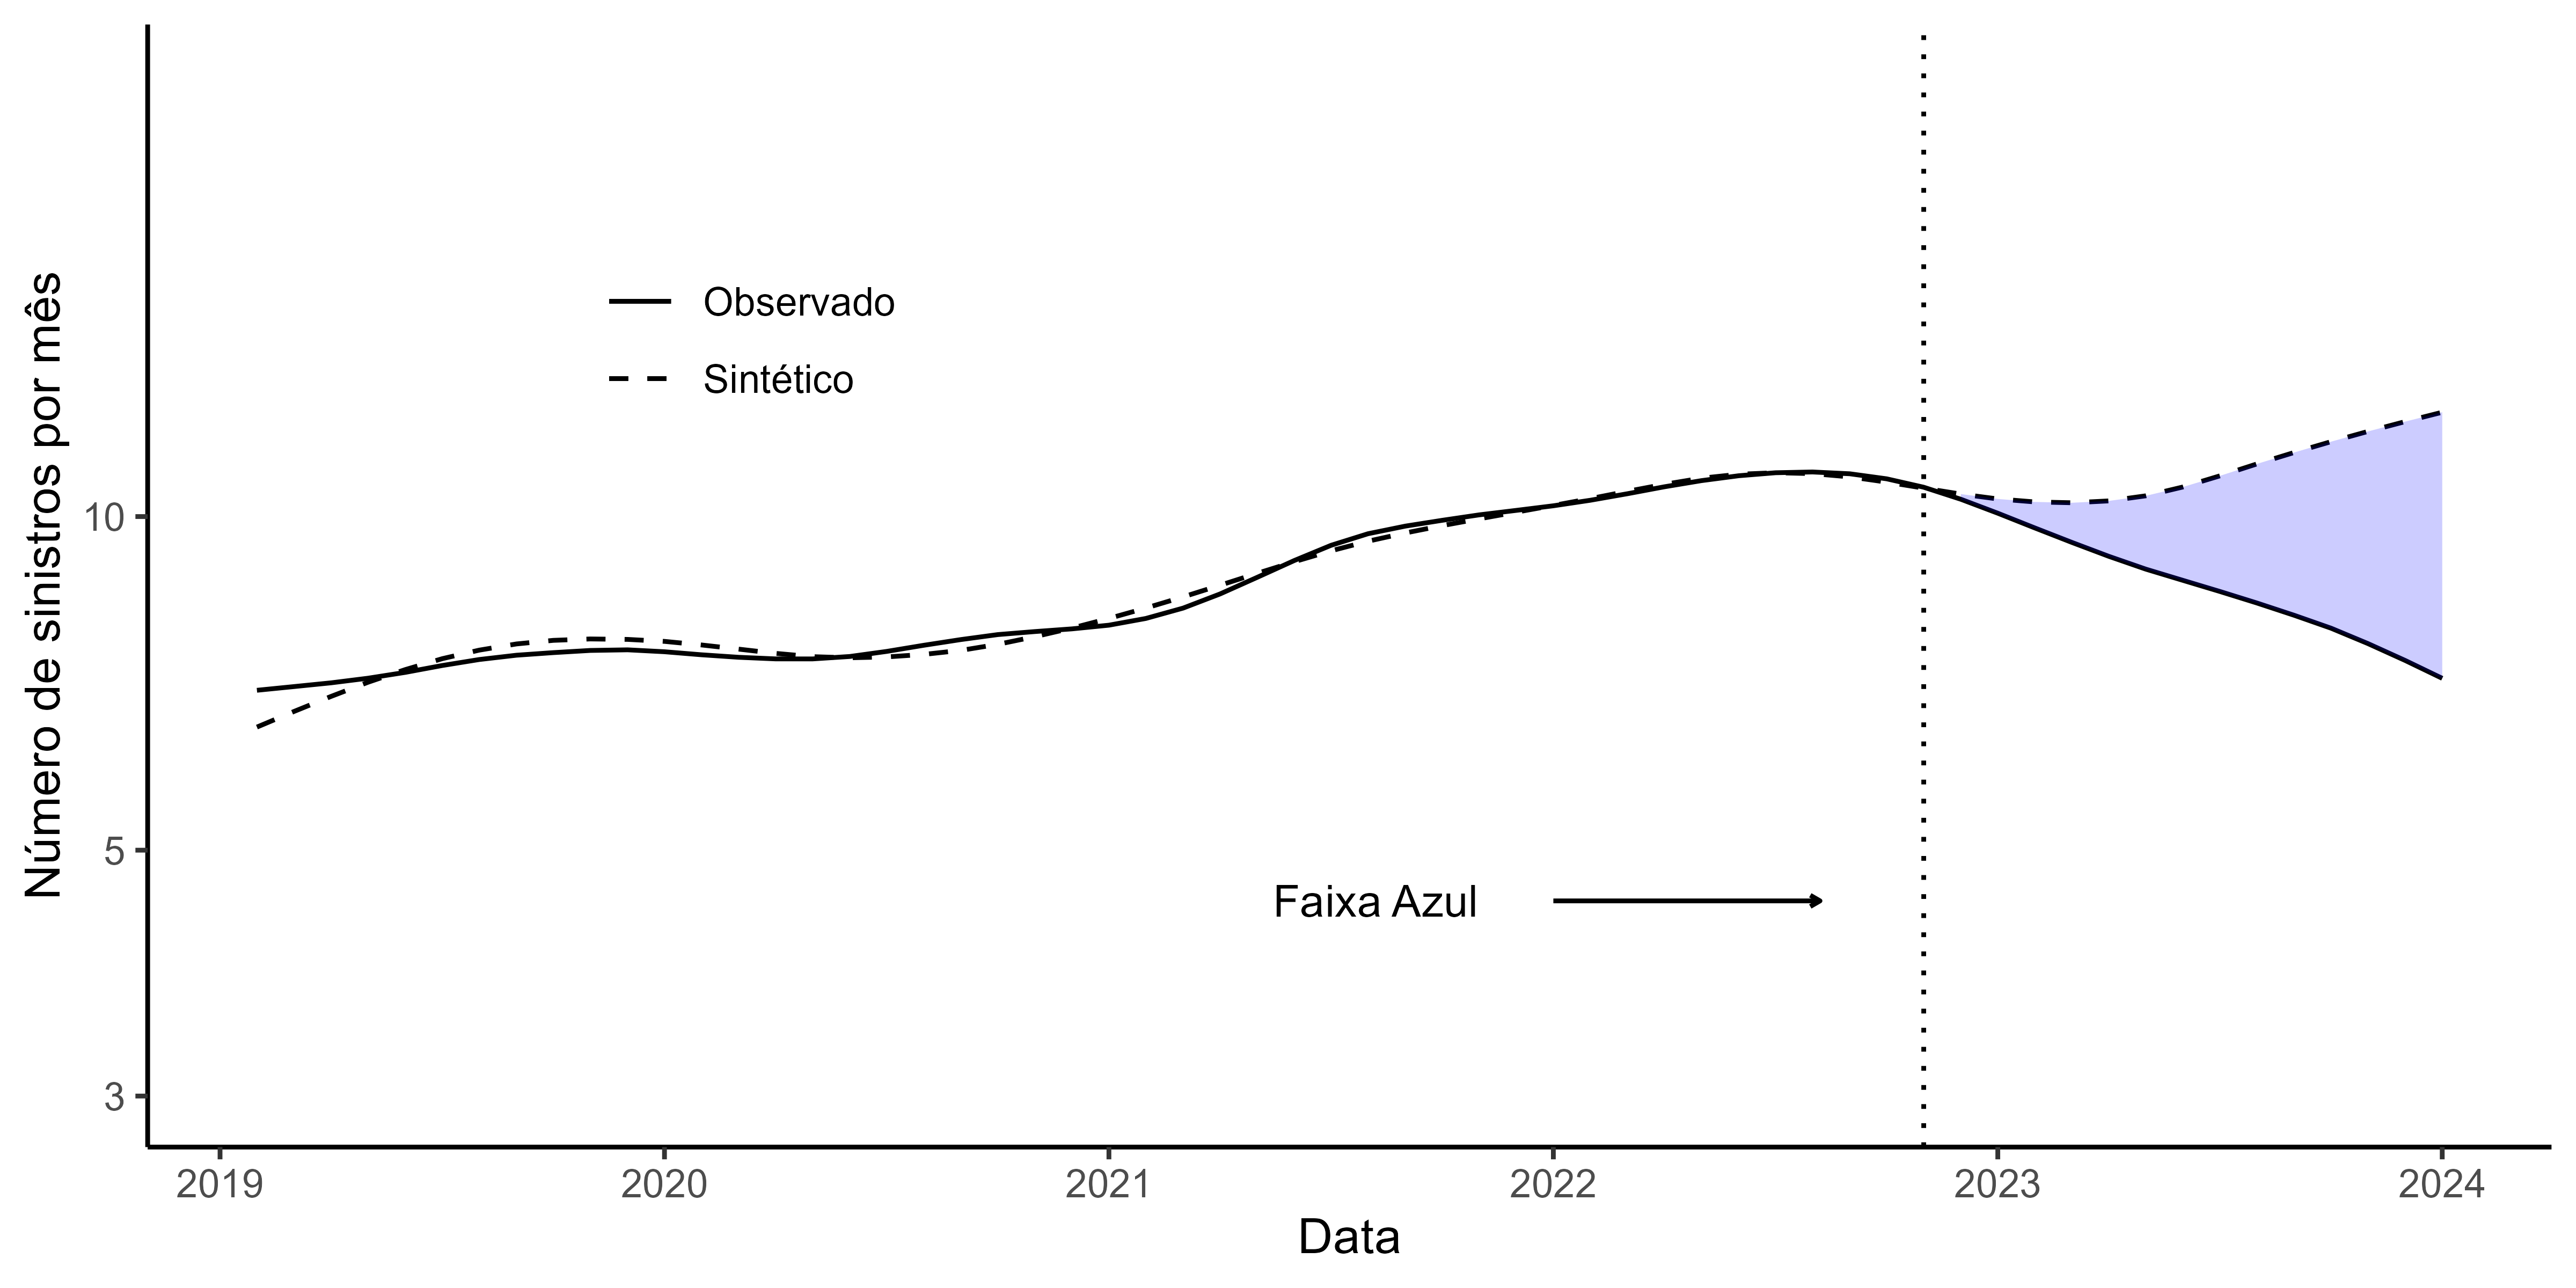
\includegraphics[width=.8\linewidth]{relatorios/faixa-azul/figuras/sintetico.png}
    \label{fig:sintetic}
\end{figure}

Caso tenha sido bem sucedido o método, com essa combinação linear de avenidas, têm-se a Bandeirantes sintética, que é igual a observada, caso esta não tivesse recebido o tratamento. O resultado pode ser visto na Figura \ref{fig:sintetic}. Dessa forma, é possível fazer uma comparação entre ambas para identificar o efeito do tratamento. A métrica utilizada para isso é o \textit{root mean squared prediction error} (RMSPE), que calcula soma da distância entre a unidade sintética e verdadeira para cada período de tempo antes do tratamento (RMSPE pré) e depois do tratamento (RMSPE pós). Essa comparação pode ser observada na Figura \ref{fig:bandeirantes_dif}. Caso o RMSPE pré seja alto, significa que o método não conseguiu formar uma unidade sintética que seja parecida com a observada, e no caso em que o RMSPE pós seja alto, isso pode ser indicativo de um efeito do tratamento. É importante destacar que ao minimizar o RMSPE pré, o método apresenta como variáveis disponíveis apenas o número de sinistros dos períodos pré tratamento. 

Como é de praxe na literatura de modelo sintético, foi feito um teste placebo para avaliar se o método identificaria efeito espúrio. Para tanto, foi considerado que o período de tratamento aconteceu 8 meses antes do real tratamento. Com isso, agora na minização do RMSPE pré, há 8 meses de dados a menos disponíveis e é possível calcular um RMSPE pós', mas apenas para os 8 meses que foram removidos (sem contar com os meses de verdadeiro tratamento). Caso esse RMSPE pós' seja maior do que do RMSPE pré, o método está identificando efeito em períodos nos quais não houve tratamento -- uma evidência de que a unidade sintética não é tão parecida com a verdadeira. Na Figura \ref{fig:bandeirantes_placebo} é possível observar que no período de 8 meses mencionadas não houve efeito, uma evidência favorável à validade do método.

\begin{figure}[h]
    \caption{Análise do controle sintético}
    \begin{subfigure}[t]{0.45\linewidth}
        \centering
        \caption{Diferença entre observado e sintético}
        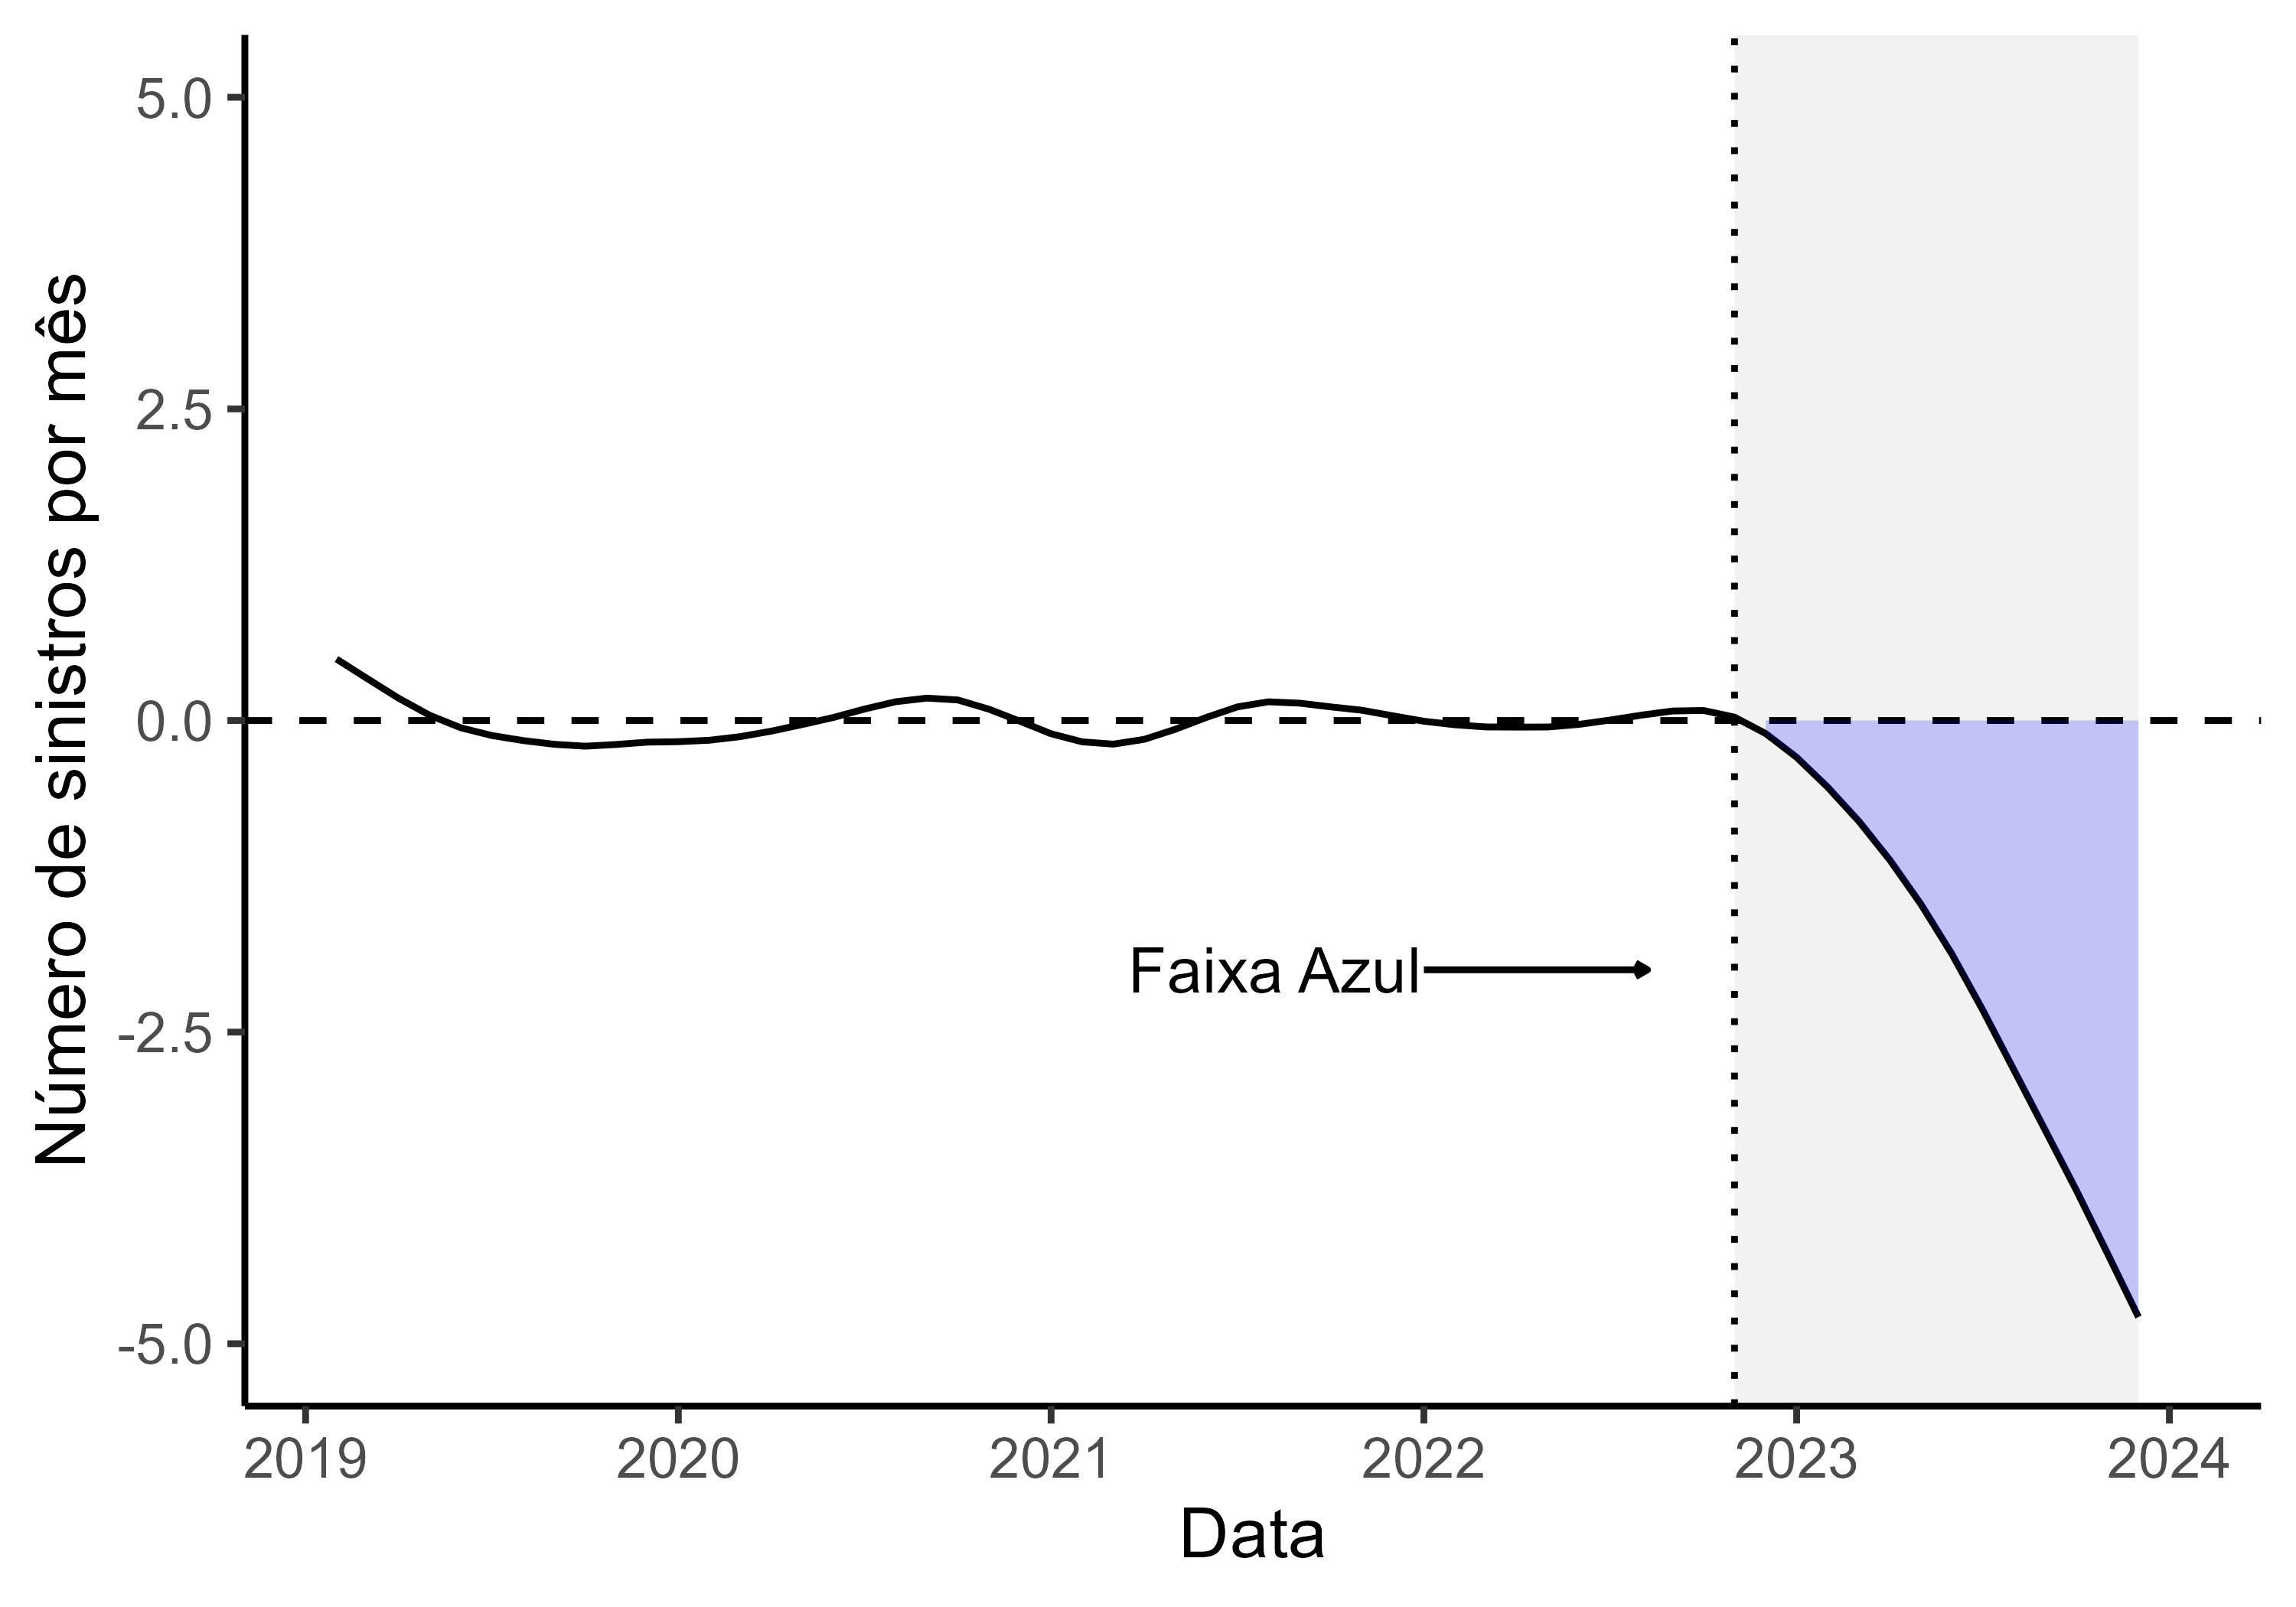
\includegraphics[width = 0.9\linewidth]{relatorios/faixa-azul/figuras/sintetico_dif.png}
        \label{fig:bandeirantes_dif}
    \end{subfigure}
    \hfill
    \begin{subfigure}[t]{0.45\linewidth}
        \centering
        \caption{Teste placebo}
        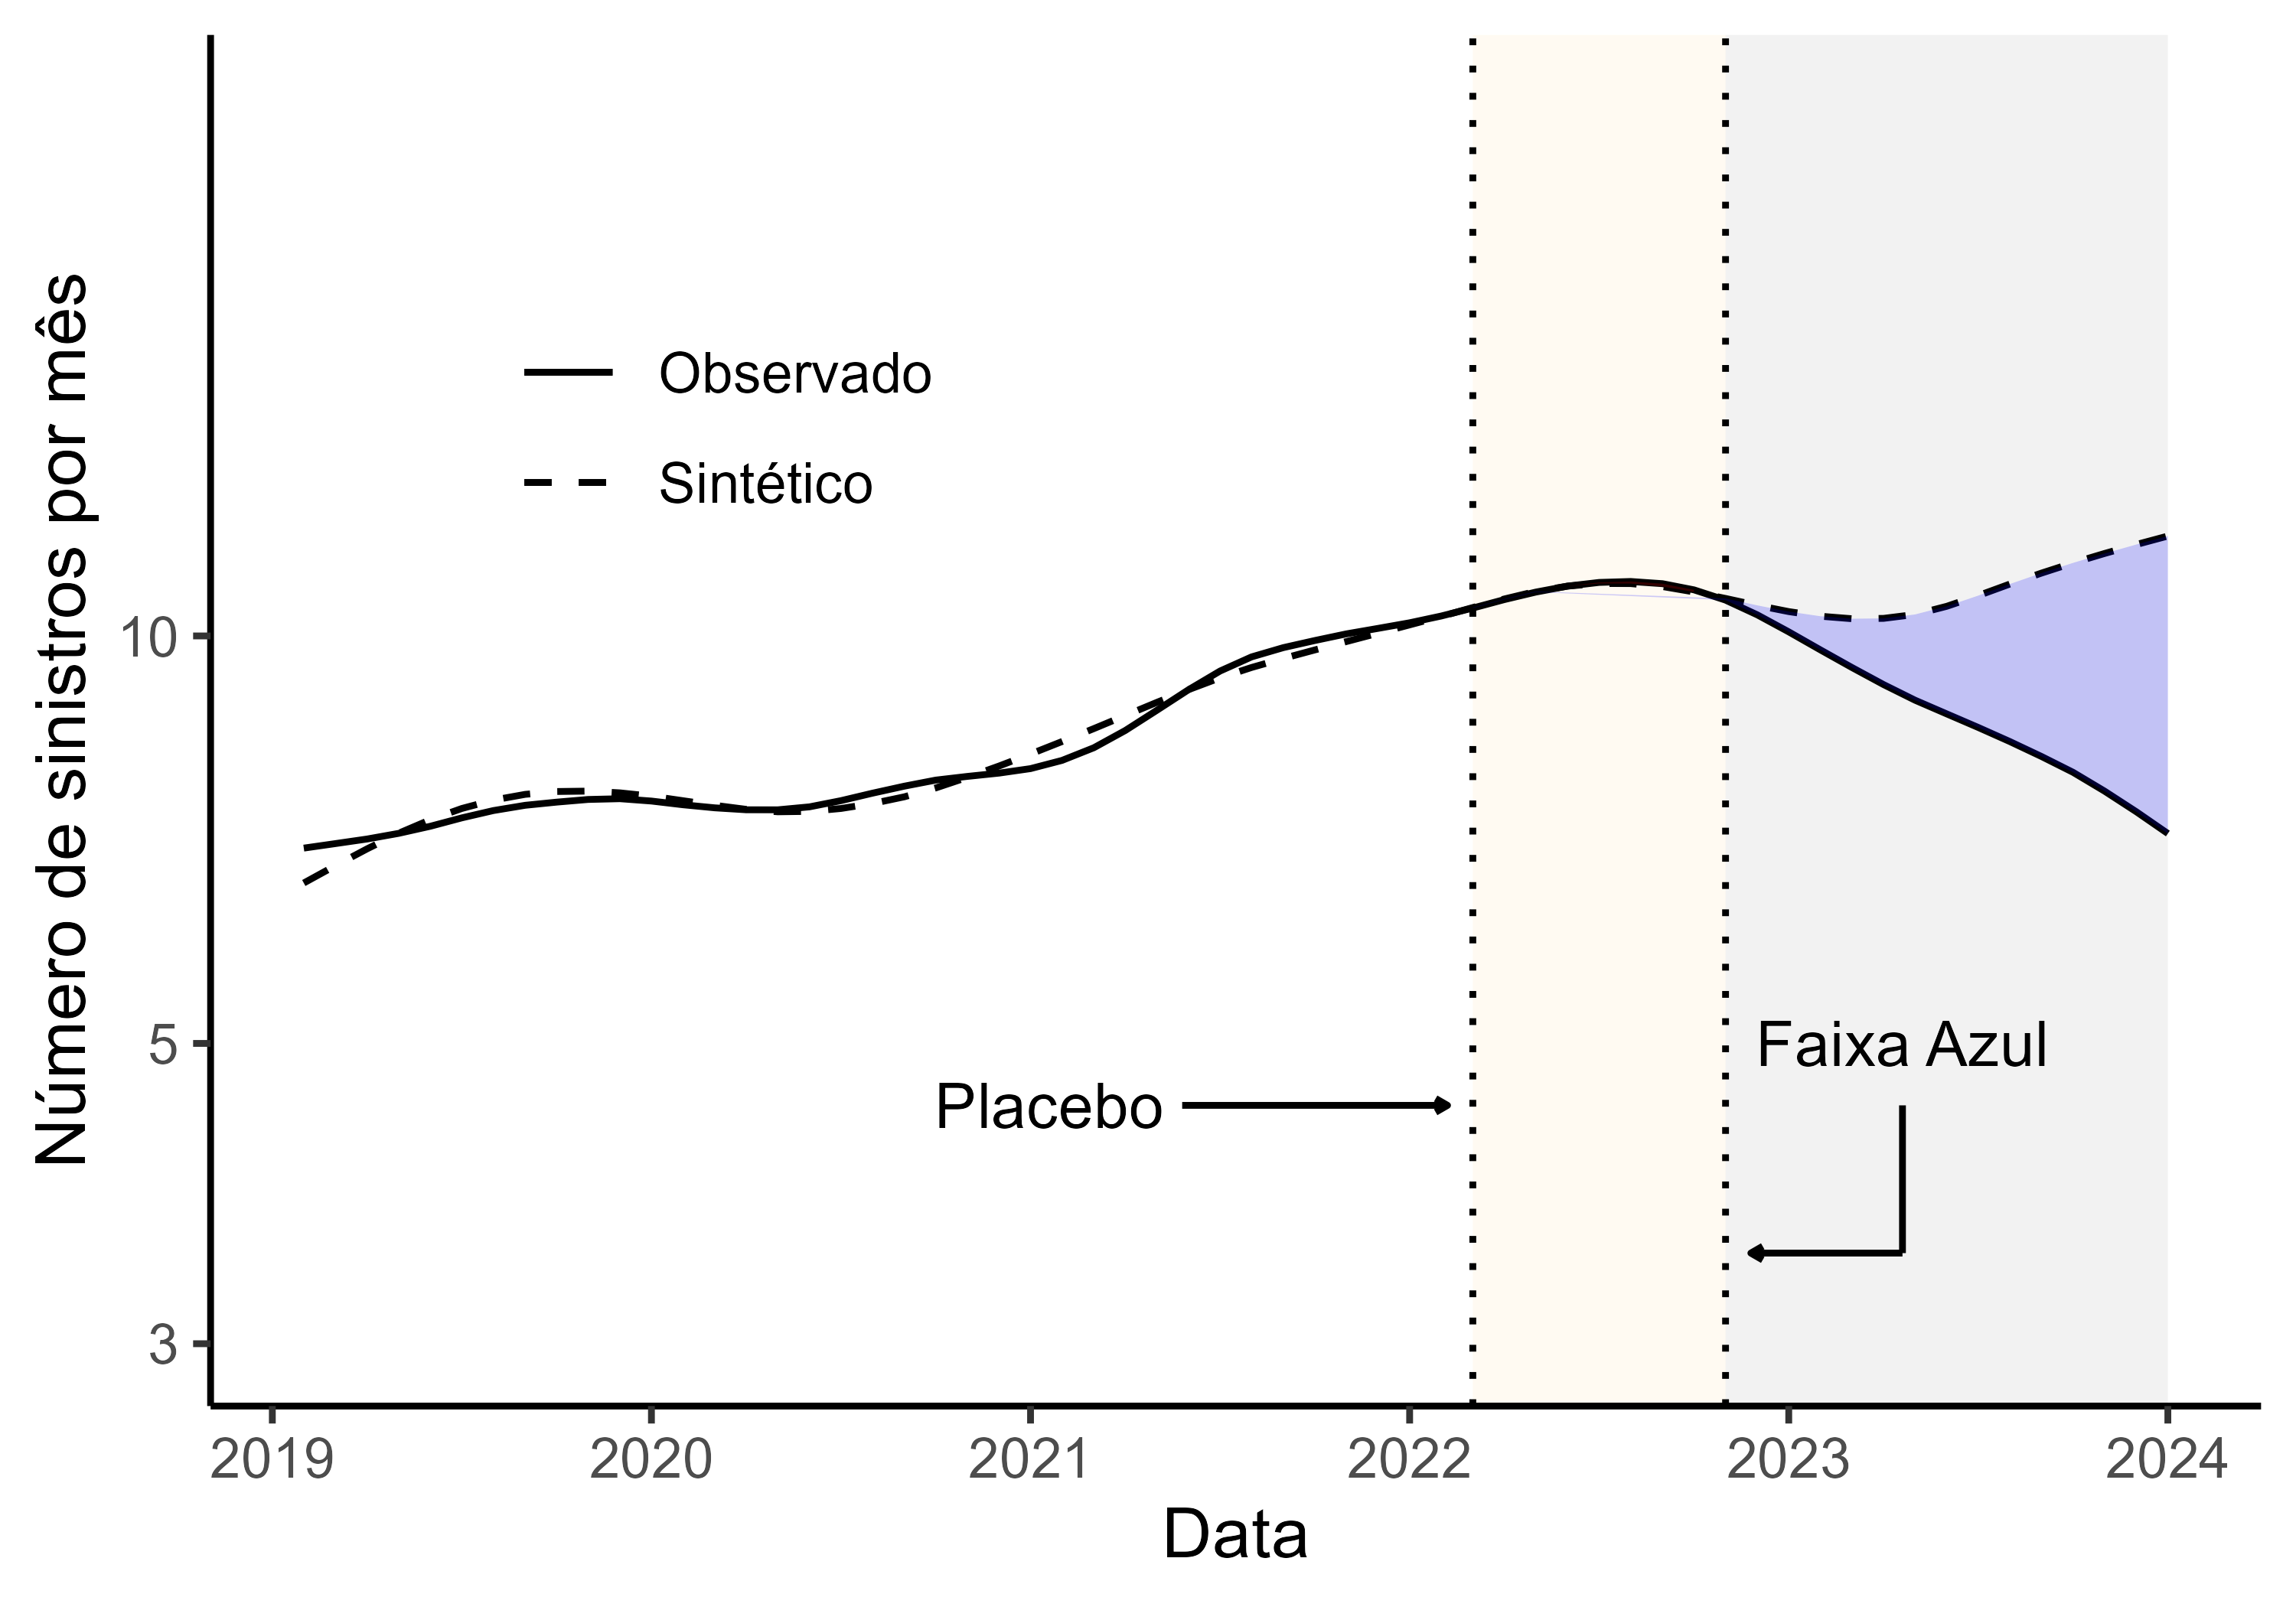
\includegraphics[width = 0.9\linewidth]{relatorios/faixa-azul/figuras/placebo.png}
        \label{fig:bandeirantes_placebo}
    \end{subfigure}
\end{figure}

Um outro tipo de teste placebo pode ser feito, no qual ao invés de manipular qual data é considerada o começo do tratamento, é possível mudar qual avenida recebeu a faixa azul -- procedimento que recebe o nome de teste da permutação. Caso se identifique efeito maior em avenidas que não receberam faixa azul, se comparadas à Bandeirantes, isso é uma evidência de que o efeito observado do tratamento na Bandeirantes pode ser espúrio, já que as outras não receberam tratamento. Para avaliar o efeito em cada avenida, é construído um controle sintético para cada uma delas que estão presentes no \textit{pool} de opções -- a mesma que foi utilizada para a construção do controle sintético da Bandeirantes. Os resultados podem ser vistos na figura \ref{fig:permutacao}. Nesse \textit{pool} foram consideradas avenidas que apresentam mais de 100 sinistros desde o início da disponibilidade de dados, resultando em 122 avenidas. 

\begin{figure}[h]
    \centering
    \caption{Resultado da permutação de controle sintético}
    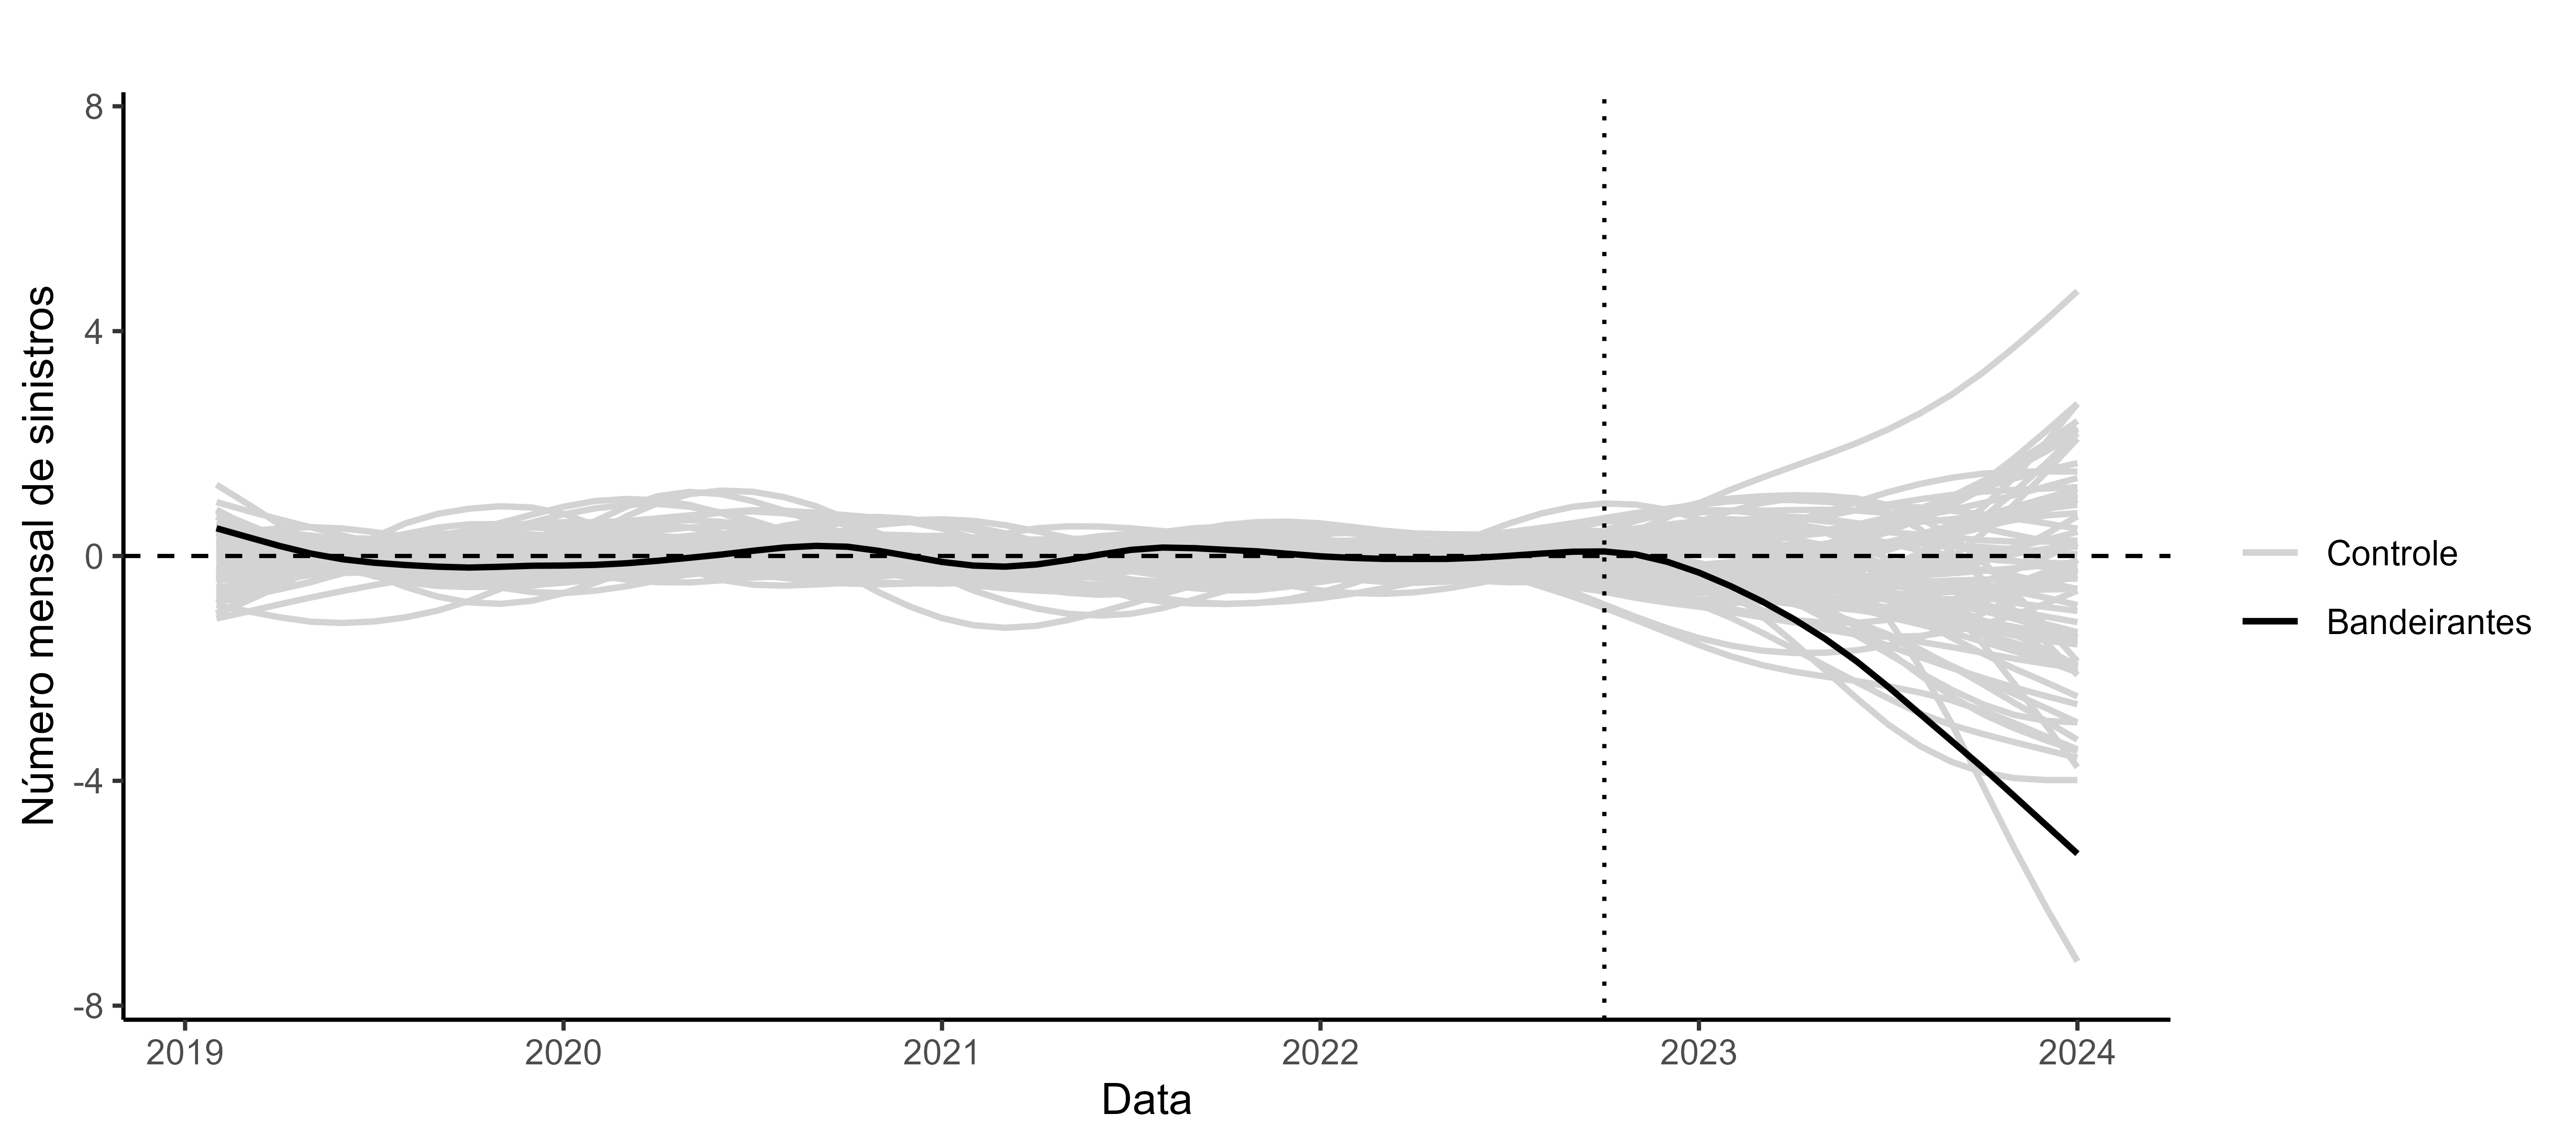
\includegraphics[width = 0.8\linewidth]{relatorios/faixa-azul/figuras/vassoura.png}    
    \label{fig:permutacao}
\end{figure}

Depois, é utilizada uma métrica na qual se divide o RMSPE pós pelo RMSPE pré para cada avenida disponivel no \textit{pool}. Quanto maior for o resultado dessa razão, mais significante é o efeito do tratamento. Entretanto, seria problemático caso unidades não tratadas tenham uma razão mais alta do que a tratada, visto que elas não receberam o tratamento. Com isso, são ranqueadas todas as unidades do \textit{pool} de maior à menor razão RMSPE pós/pré. Com base nesse ranqueamento, é calculado o p-valor do método. 

\begin{figure}[h]
    \centering
    \caption{Ranqueamento das razões RMSPE pós/pré}
    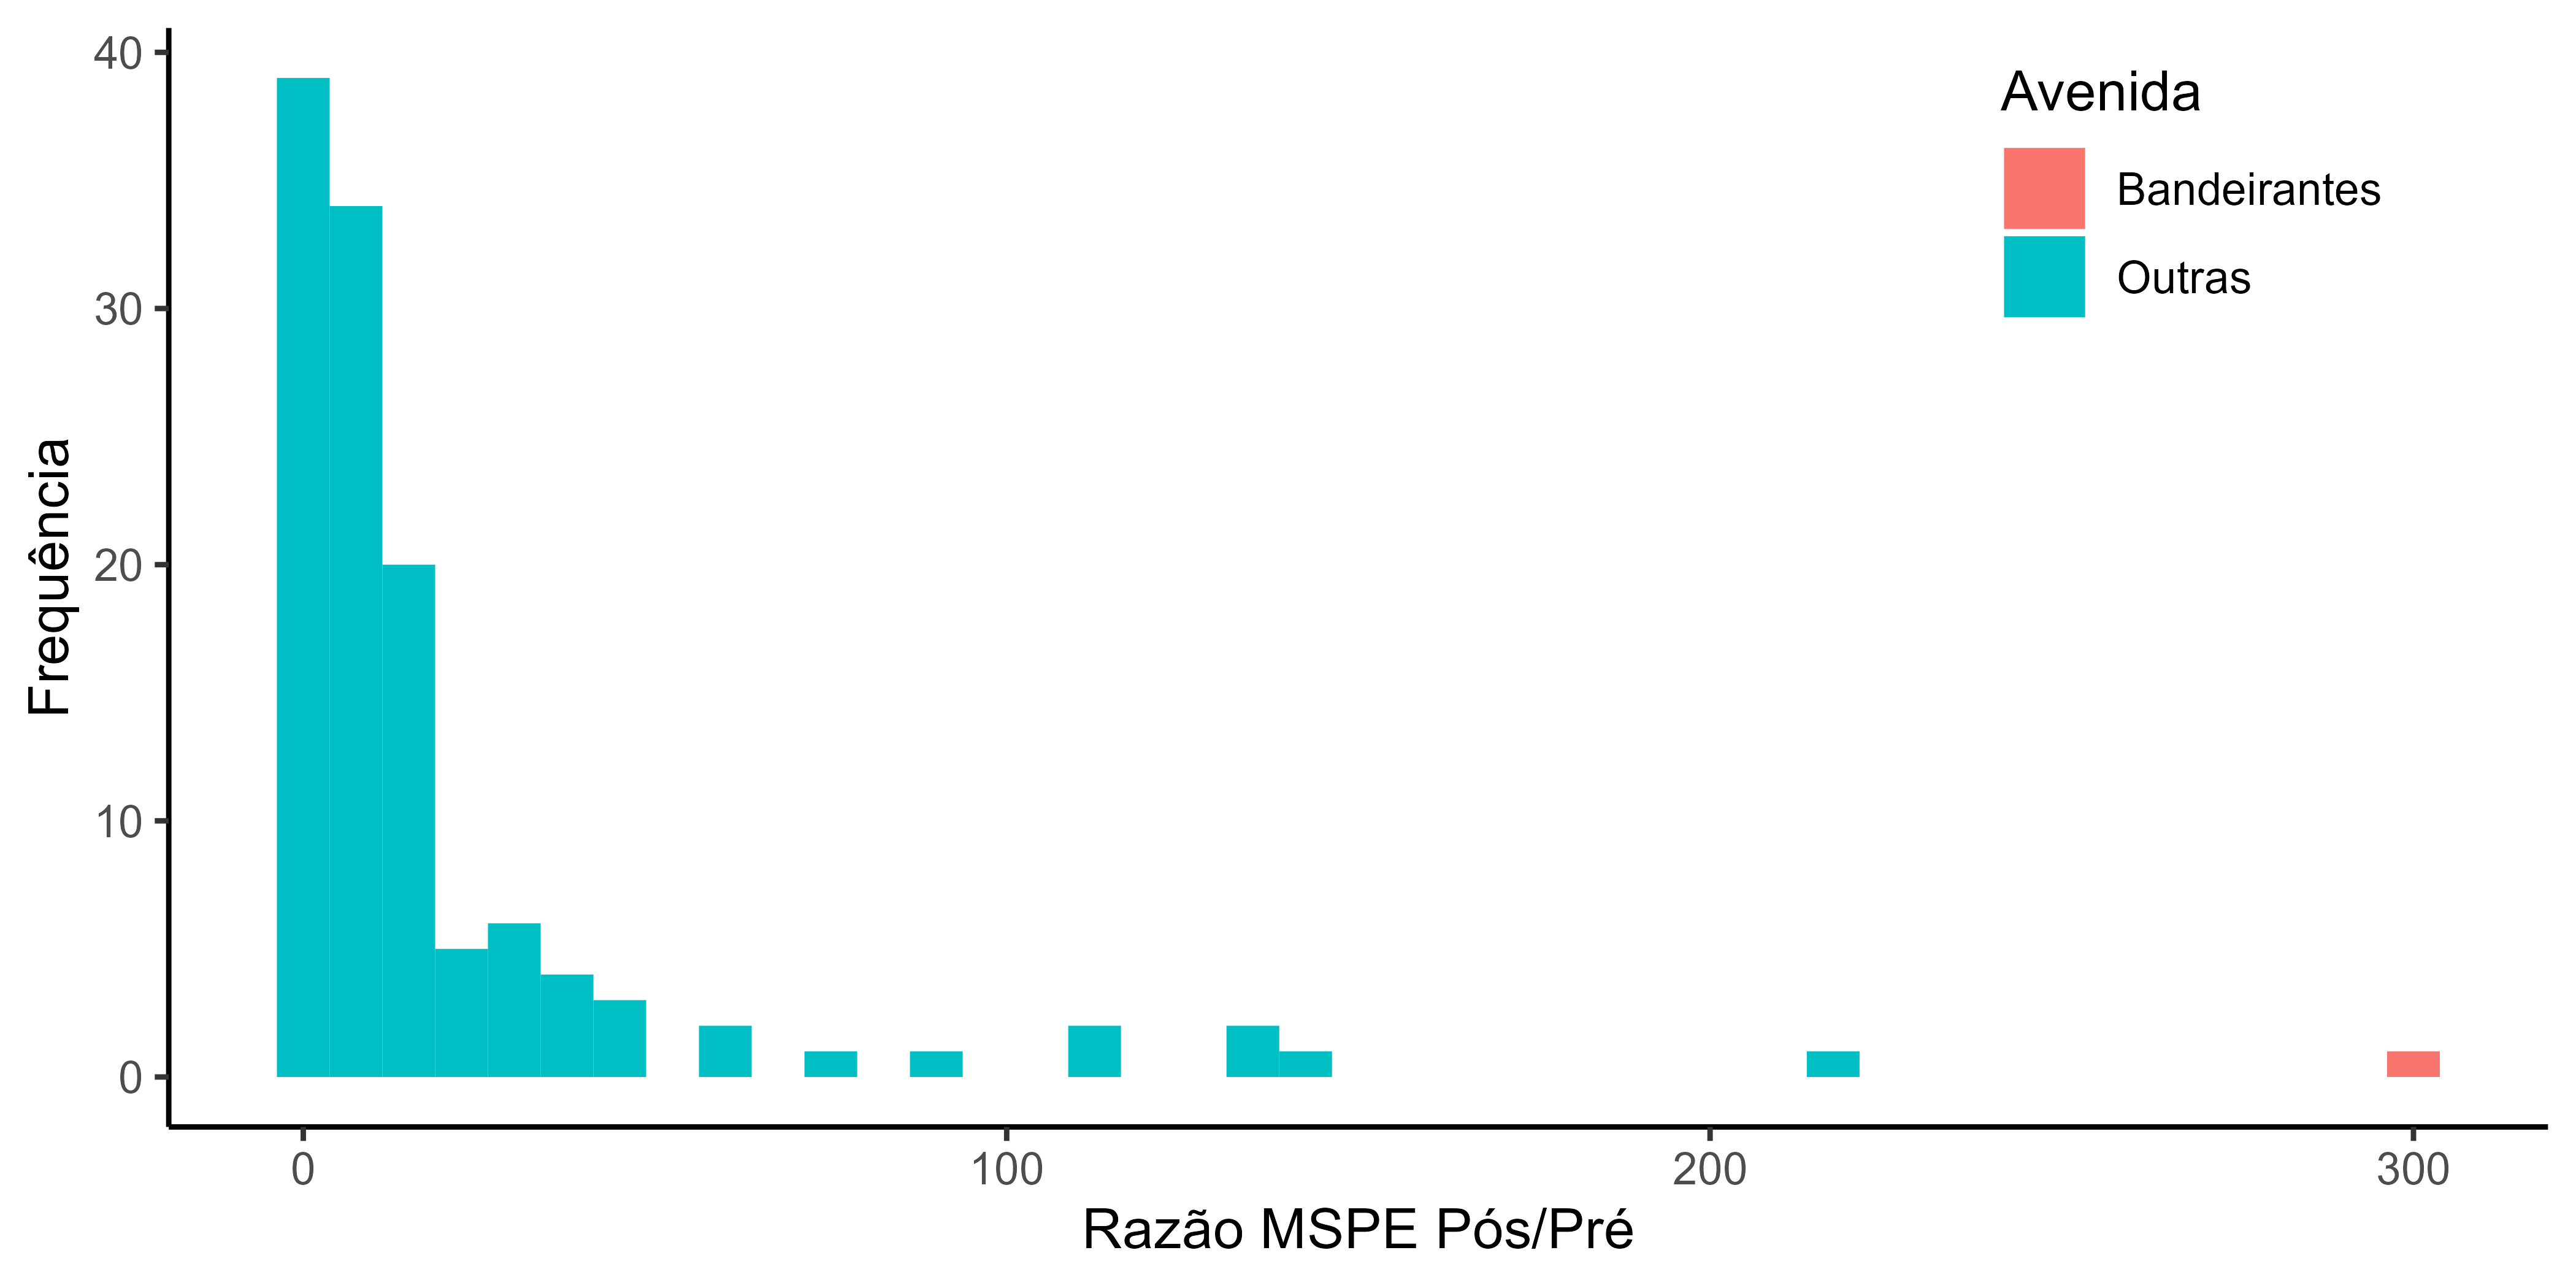
\includegraphics[width = 0.7\linewidth]{relatorios/faixa-azul/figuras/histograma_ratio.png}    
    \label{fig:ranqueamento}
\end{figure}

Como é possível observar na Figura \ref{fig:ranqueamento}, a Avenida dos Bandeirantes ficou em primeiro lugar no ranking, o que é um forte indicativo de que a medida foi bem sucedida. É possível fazer uma interpretação semelhante ao clássico p-valor das estatísticas construídas com regressões lineares. Caso fosse amostrada uma nova avenida a partir da permutação aleatória de avenidas da \textit{pool}, a probabilidade de uma apresentar o mesmo ou maior efeito, se comparada à Bandeirantes é $1/122$, que equivale a um ``p-valor'' de 0.82\%. Entretanto, essa \textit{pool} pode ser considerada muito grande e com avenidas que não tiveram um bom controle sintético formado. Nesse sentido, a literatura recomenda a remoção de unidades amostrais com erros pré-tratamento muito grandes.

Em \textcite{abadie2010synthetic}, é colocado como valor de corte as unidades da \textit{pool} que apresentaram erro pré-tratamento 20 vezes maior do que a unidade tratada, sendo considerada uma \textit{lenient cutoff} pelos autores. Quanto mais leniente for o valor de corte, mais significativo se torna o efeito da faixa azul. Quando imposto este limite, o novo p-valor torna-se 1.35\%, já com um limite de 10 vezes a unidade tratada (uma medida mais conservadora), têm-se um p-valor de 2.22\%.




